% !TeX root = ../main.tex
% Add the above to each chapter to make compiling the PDF easier in somexcv editors.

\chapter{State of the Art}\label{chapter:theoretical_background}

Machine Learning \cite{wang2016machine, mahesh2020machine} is a rapidly evolving field of artificial intelligence. There are different types of algorithms that are used for specific tasks involving supervised learning where the algorithm maps inputs to the given labels, unsupervised learning where the labels to the input are not available, and semi-supervised learning which combines labelled and unlabeled data. Additionally, there is reinforcement learning where the model learns by observing the environment \cite{ayodele2010types}. Specific tasks are e.g. classification where the input has to be assigned to specific classes, regression where the input has to be assigned to a continuous value (both supervised) and clustering (unsupervised) where the goal is to group the input. 

There are many different algorithms that accomplish these goals, for example support vector machines \cite{noble2006support}, the tsetlin machine \cite{granmo2018tsetlin}, and decision trees \cite{rokach2005decision}. One very important class of algorithms is \textit{artificial neural networks} \ref{sec:neural_networks}. After the introduction to neural networks, hyperparameter optimization is presented with different techniques to improve machine learning models. In the following, sparse grids are presented which will be needed as a foundation for hyperparameter optimization of neural networks with sparse grids. 

\section{Introduction to Neural Networks}\label{sec:neural_networks}

Neural networks \cite{bishop1994neural, da2017artificial} are very powerful for solving various tasks. They are very versatile and they exist in very different variations, ranging from a very small size up to very large networks for more complex tasks.

The smallest part of a neural network is the \textit{perceptron}. A network consisting only of one perceptron can be seen in Figure \ref{fig:perceptron}.

\begin{figure}[H]
	\centering
	\def\svgscale{0.5}
	\input{figures/drawing.pdf_tex}
	\caption{ Neural network consisting of only one perceptron. The output is computed according to Equation \ref{eq:perceptron}.}
	\label{fig:perceptron}
\end{figure}

The output $ y $ is computed with 

\begin{equation}
	\label{eq:perceptron}
	u = \sum_{i=1}^n w_i \cdot x_i - \theta  \text{,   } y = g(u).
\end{equation}

The network has $ n $ inputs $ x_i $ and weights $ w_i $. $ \theta $ is the activation threshold (also called bias), $ g $ is the activation function, and $ u $ is the activation potential \cite{da2017artificial}. 

This basic building block can then be used to build a more complex architecture with multiple layers. All neural networks have an input layer consisting of $ n \in \mathbb{N}$ input neurons and an output layer with $ m \in \mathbb{N} $ output values. Between them, there can be multiple hidden neural layers. In deep neural networks, this number of layers is very high as the name suggests. Each neuron of each layer again has weights of the corresponding input and bias. The concrete values for them are important for the behavior of the model and determine the performance. These values are learned during the training phase of the model. There are two stages (forward and backward stage) during the training phase as can be seen in Figure \ref{fig:network}.

\begin{figure}[H]
	\centering
	\def\svgscale{0.5}
	\input{figures/drawing2.pdf_tex}
	\caption{ Neural network consisting of two hidden layers. The connections between the perceptrons are bidirectional. In the forward phase, the intermediate results are given to the neurons to the right and in the backward phase from right to left. }
	\label{fig:network}
\end{figure}

The figure shows a schematic neural network with two hidden layers and $ n_1 $ neurons in the first layer and $ n_2 $ ones in the second layer. In the forward stage, an input $ x \in \mathbb{R}^n $ is put into the network and the output is computed by computing the corresponding result of each neuron and feeding it into the next layer to the right according to the connections. This output is then taken to update the weights of all neurons in the backward stage. In the simple case depicted in Figure \ref{fig:perceptron} with only one perceptron, the weights are updated with  

\begin{equation}
	\label{eq:weights_update}
	w_{current} = w_{previous} + \eta \cdot \left(d^{(k)} - y\right) \cdot x^{(k)}
\end{equation}

where $ w = [\theta \text{ } w_1 \text{ } ... w_n]^T $ is the vector with all weights and the bias, $ x = [-1 \text{ } x_1^{(k)} \text{ } ... x_n^{(k)}]^T $ is the $ \text{k}^{\text{th}} $ training sample, $ d^{k} $ the desired label, $ y $ the output of the perceptron and $ \eta $ the learning rate. The choice of $ \eta $ is fixed before training and usually $ 0 < \eta < 1 $. For the update of the weights of networks with multiple layers, refer to \cite{da2017artificial}. 

The perceptron and its training is the basic building block for most neural networks. Based on this, the concrete architecture can still be adjusted. One first thing is to increase the number of layers or neurons per layer. But also the choice of connections between layers can improve the performance of the network. Another thing that can be done is to introduce connections from higher layers to lower layers which makes it a recurrent neural network. They are especially suited for sequential or time-varying patterns \cite{medsker2001recurrent}. There is also a specific architecture for grid-structured data like images. For them, convolutional neural networks are used to extract features \cite{li2021survey, gu2018recent, o2015introduction}. For further readings on different architecture choices, refer to \cite{liu2017survey}.

In all cases, the weights of the network are updated automatically and it is impossible to understand the concrete decision-making of the model. The weights are called parameters of the network. Besides them, there are hyperparameters that have to be fixed before training. They are design decisions on how the network should behave. For some of them, experience can show which choices lead to better performances of the model but in all cases, they can be optimized which will be discussed in the following section \ref{sec:hyperparameter_optimization}. Some of the hyperparameters are
\begin{itemize}
	\item Epochs: Number of times the training data is fed into the network and the weights are updated
	\item Learning rate: $ \eta $ of Equation \ref{eq:weights_update} defining how fast the model should learn
	\item Optimizer: Optimizer used to update the weights of the network
	\item Loss function: Concrete loss metric how the label and the output are compared in Equation \ref{eq:weights_update}
	\item Batch size: Number of data samples processed in a batch
	\item Number of layers of the network
	\item Number of neurons in each layer
\end{itemize}

All these parameters can drastically influence the model performance. In the following section, different techniques for the optimization are presented.


\section{Hyperparameter Optimization}\label{sec:hyperparameter_optimization}

Most machine learning models have parameters that have to be defined before the learning phase. They are called hyperparameters and strongly influence the behavior of the model. One example is the number of epochs of the learning phase of a neural network. There are different techniques for the optimization of hyperparameters and they all define the machine learning model as a black box function $ f $ with the hyperparameters as input and the resulting performance as output. The overall goal is to find a configuration $ \lambda_{min} $ from $ \Lambda = \Lambda_1 \times \Lambda_2 \times ... \times \Lambda_N $ that minimizes the function $ f $ with $ N $ hyperparameters with 
\begin{equation}
	\label{eq:optimization}
	\lambda_{min} = \text{arg} \min_{\lambda \in \Lambda} f(\lambda) .
\end{equation}

In our case, the function f is a machine learning algorithm that is trained on a training set and evaluated on a validation set. With this, the minimization of e.g. the loss of the model optimizes the decisions it is making which leads to better prediction results. Note that one function evaluation of f is usually very expensive as the training of a machine learning model with many parameters and weights takes much time. The data set consists of $ \left\{ (x_i, y_i) | x_i \in X, y_i \in Y, 0 \le i \le m \right\} $ with m being the number of data samples. The $ x_i $ is the input data to the model and the goal is that 
\begin{equation}
	\forall i: M(x_i) = y_i.
\end{equation}
where M is the model. In the context of supervised learning, the whole data set is split into a training set which is used to optimize the model and a testing set to evaluate the performance on new, unseen data \cite{supervised_learning}.

In summary, the goal is get evaluation scores on the testing data set which can be achieved with Equation \ref{eq:optimization}. 
\cite{feurer2019hyperparameter,bischl2021hyperparameter,yang2020hyperparameter}

In the following, different techniques for the optimization are presented and discussed with their advantages and disadvantages.

\subsection{Grid Search}
The idea of the first approach for optimization is to discretize the domains of each hyperparameter and evaluate each combination. This suffers from the curse of the dimensionality as it scales exponentially with the number of hyperparameters. For $ d $ parameters and $ n $ values per hyperparameter, $ n^d $ different configurations are possible which all have to be evaluated. 

One advantage of this method is that it is easy to implement and very simple. Also, the whole search space is explored evenly.

On the other hand, the curse of the dimensionality makes it very slow if the function evaluations are very expensive which is the case for most machine learning algorithms. Another drawback is that each hyperparameter only takes $ n $ different values. The comparison to random search can be seen in Figure \ref{fig:comparison_searches}.


\subsection{Random Search} \label{Random_search}
The next technique \cite{random_search} is similar to the grid search because the idea is also to evaluate different hyperparameter configurations. In contrast to the previous one, random search generates for each run and for each parameter exactly one random value from an interval which has to be specified. For this approach, a budget $ b $ has to be given. This parameter determines the number of different combinations that are evaluated. A direct comparison of grid search and random search can be seen in figure \ref{fig:comparison_searches}.

\begin{figure}[H]
	\centering
	%\includegraphics[scale=0.2]{figures/comparison_searches.png}
	\includegraphics[width=0.9\textwidth]{figures/Fig_2_3_grid_random_search}
	\caption{Comparison of grid search (left) and random search (right) in the two dimensional case. For both techniques, 9 different combinations are evaluated. In the left case, only 3 distinct values for each hyperparameter are set whereas there are 9 different values for each parameter in the random search. }
		% Taken from \cite{feurer2019hyperparameter}. }
	\label{fig:comparison_searches}
\end{figure}

In this figure, a two-dimensional setting is depicted. For both techniques, 9 different combinations are evaluated. In the case of grid search, only 3 distinct values are taken for each hyperparameter while there are 9 different ones in the random search. In this example, the better result is found in random search as more distinct values are taken for the important parameter. Note that it is not always the case that random search leads to better results.

Compared to the normal grid search, this is one advantage. For each hyperparameter, $ b $ (budget) different values are taken into consideration which is much more compared to the grid search with the same overall number of combinations. Additionally, this technique is also easy to implement and relatively simple. 

One disadvantage is that it is also very expensive if the budget is high because of the long training times of machine learning models. 


\subsection{Bayesian Optimization}

Another possible technique for finding the best hyperparameters of machine learning models is called bayesian optimization (BO) \cite{snoek2012practical}. This is an iterative approach for optimizing the expensive black box function by modelling it based on observations. A so-called \textit{surrogate model} $ \hat{f} $ is made with the help of the \textit{archive} $ A $ which contains observed function evaluations. This surrogate model is created by regression and the technique which is most often used is the Gaussian process \cite{bischl2021hyperparameter} which is only suitable if the number of hyperparameters is not too high \cite{andonie2019hyperparameter}. The problem of this technique arises when some hyperparameters are categorical or integer-valued which is the reason why extra approximations can lead to worse results and special treatment is needed \cite{garrido2020dealing}. Another possible technique for the surrogate model is using random forests \cite{hutter2011sequential}. All in all, this function estimates the machine learning model depending on the hyperparameter configuration and also the prediction uncertainty $ \sigma(\lambda) $. A second function called \textit{acquisition function} $ u(\lambda)$ is built based on the prediction distribution. This $ u $ is responsible for the trade-off between exploitation and exploration. This means that configurations that lead to better model performances are exploited and values where not much information is gathered are explored. There are many numerous different possibilities for this function  \cite{wilson2018maximizing} but the most used one is the \textit{expected improvement} (EI) which is calculated with

\begin{equation}
	E[I(\lambda)] = E\left[max\left(f_{min}-y, 0\right)\right].
\end{equation}

If the model prediction y with configuration $ \lambda $ follows a normal distribution \cite{feurer2019hyperparameter}, it leads to 

\begin{equation}
	E[max\left(f_{min}-y\right), 0] = \left(f_{min}-\mu(\lambda)\right) \Phi\left(\frac{f_{min}-\mu(\lambda)}{\sigma}\right) + \sigma \phi \left(\frac{f_{min}-\mu(\lambda)}{\sigma}\right)
\end{equation}

with $ \phi $ and $ \Phi $ being the standard normal density and standard normal distribution and $ f_{min} $ the best result so far. 


In each iteration, a new candidate configuration $ \lambda^+ $  is generated by optimizing the acquisition function $ u $. This $ u $ is much cheaper to evaluate than the $ f $ which includes learning of an expensive neural network which makes the optimization much easier.

The exact steps are presented in Algorithm \ref{alg:bayesian_opt} and Figure \ref{fig:bayesian_optimization} shows schematic iteration steps.

\begin{algorithm}[H]
	\caption{Bayesian Optimization for a black box function f. In each iteration, the surrogate model is fitted on the current archive and an acquisition function is built. The optimum of this acquisition function is evaluated and added to the archive.}
	\label{alg:bayesian_opt}
	\begin{algorithmic}
		\State Generate initial $\lambda^{(1)}, ..., \lambda^{(k)} $
		\State Initialize archive $A^{[0]} \gets \left(\left(\lambda^{(1)}, f\left(\lambda^{(1)}\right)\right), ..., \left(\lambda^{(k)}, f\left(\lambda^{(k)}\right)\right)\right)$
		\State $ t \gets 1 $ 
		\While{Stopping criterion not met}
			\State Fit surrogate model $ \left(f(\lambda), \sigma(\lambda)\right) $ on $ A^{[t-1]} $
			\State Build acquisition function $ u(\lambda) $ from $ \left(\hat{f}\left(\lambda\right), \sigma(\lambda)\right) $
			\State Obtain proposal $ \lambda^{+} $ by optimizing $ u: \lambda^+ \in arg\max_{\lambda \in \Lambda} u(\lambda) $
			\State Evaluate $ f\left(\lambda^+\right)$
			\State Obtain $A^[t]$ by augmenting $ A^{[t-1]} $ with $ \left(\lambda^{(+)}, f\left(\lambda^{(+)}\right)\right) $
			\State $ t \gets t+1 $
		\EndWhile
		\State return $ \lambda_{best} $: Best-performing $\lambda$ from archive or according to surrogates prediction
	\end{algorithmic}
\end{algorithm}

\begin{figure}[H]
	\centering
	%\includegraphics[scale=0.35]{figures/bayesian_optimization.png}
	\includegraphics[width=\textwidth]{figures/Fig_2_4_bayesian}
	\caption{ Schematic iteration steps of the bayesian optimization. The maximum of the acquisition function determines the next function evaluation (red dot in the middle). The goal is to find the minimum of the dashed line. The blue band is the uncertainty of the function. }
		%Taken from \cite{feurer2019hyperparameter}. }
	\label{fig:bayesian_optimization}
\end{figure}


First, $ k $ initial hyperparameter configurations are sampled and evaluated. This set is the starting archive $ A^{[0]} $. After that, the loop is executed as long as the stopping criterion is not met. This can be for example a budget, meaning a maximum number of function evaluations. The first step of the loop is to fit the surrogate model on the current archive. Then the acquisition function is made and optimized to get the next configuration $ \lambda^+ $. This point is evaluated and added to the archive. The overall result of the algorithm is the $ \lambda $ which is the hyperparameter configuration for the machine learning model with the overall best result.

\subsection{Other Techniques}
There are also other techniques for finding the best hyperparameters. Multi-fidelity optimization \cite{feurer2019hyperparameter} aims to probe the learning of a model on a task with reduced complexity such as a subset of the data or fewer epochs for training the model for discovering the best configurations. For example, the learning curve can be predicted so that early stopping can be done if the prediction is not as good as the best model so far. There are also bandit-based selection methods that do not predict the learning curve but compare the different combinations on a small number of epochs and only perform the best ones. This can be done iteratively like it is done in \textit{successive halving} for hyperparameter optimization \cite{jamieson2016non}. The algorithm is very simple. It starts to evaluate all different combinations with a very small budget. The best half of the candidates are then evaluated in the next iteration with a double budget and so on until only one combination is left. In \cite{8030298}, a similar algorithm is presented. The authors use a model of the objective function (neural network depending on configurations) to find candidate hyperparameters. Those are then trained on a smaller number of epochs and the best ones are then evaluated with a higher budget. Also, neural networks can be used for the optimization which was done by the authors in \cite{smithson2016neural}. Also, the covariance matrix adaptation evolution strategy was implemented as an alternative to bayesian optimization in \cite{loshchilov2016cma}. 


\section{Sparse Grids}

Sparse grids are a useful tool to mitigate the \textit{curse of the dimensionality} by reducing the number of grid points. In the following, this technique is presented after the general numerical approximation of functions.

\subsection{Numerical Approximation of Functions}

Let $ f: \Omega \rightarrow R $ be a function defined on the unit interval $ \Omega = [0,1]^d $ in $ d $ dimensions. For simplicity, we first set $ d=1$. Now this function can be represented on a grid of level $ l \in \mathbb{N}_0 $ with $ 2^l + 1 $ grid points which are 
\begin{equation}
	x_{l,i} = i*h_l, \text{   } i = 0,...,2^l,
\end{equation}

with i being the index and $ h_l = 2^{-l} $ being the distance between the grid points. Each of them gets a basis function defined by 
\begin{equation}
	\varphi_{l,i}: [0,1] \rightarrow \mathbb{R}.
\end{equation}

There are different possibilities for the basis functions which will be presented later. For the simplicity, we present a simple example being the hat function defined by
\begin{equation}
	\varphi_{l,i}(x) = \max\left(1- \left|\frac{x}{h_l}-i\right|, 0\right).
\end{equation}
All in all, the space of functions that can be presented exactly by a linear combination is called the \textit{nodal space} $V_l$ with the assumption that the basis functions form a basis:
\begin{equation}
	V_l = \text{span}\left\{ \varphi_{l,i} | i = 0,...,2^l\right\}. 
\end{equation}

Every function $f: [0,1] \rightarrow \mathbb{R}$ can be interpolated by a the interpolant $ u $ defined by
\begin{equation}
	f_l = \sum_{i=0}^{2^l}\alpha_{l,i} \varphi_{l,i}, \forall i = 0,...,2^l: f_l(x_{l,i}) = f(x_{l,i})
\end{equation}

for constants $ \alpha_{l,i} \in \mathbb{R} $. An example can be seen in Figure \ref{fig:interpolant}.


\begin{figure}[H]
	\centering
	\includegraphics[width=\textwidth]{figures/Fig_2_5_interpolant}
	\caption{  Interpolation of the function $ f $ (black line) by its interpolant $ u $ (red, dashed) in the nodal basis. Level of the grid is 3 and hat functions are used. }
	\label{fig:interpolant}
\end{figure}

%\begin{figure}[H]
%	\centering
%	\includegraphics[scale=0.5]{figures/weighted_sum.png}
%	\caption{ Interpolation of the function $ f $ (black line) by its interpolant $ u $ (red, dashed) in the nodal basis. Level of the grid is 3 and hat functions are used. Taken from \cite{pfluger2010spatially}. }
%	\label{fig:interpolant}
%\end{figure}

On the left side, the function f (black line) can be seen with a grid of level 3. On the right side, the interpolant u as a linear combination of the basis functions (hat functions centered on the grid points) can be seen. This approach is the nodal basis. The second possibility is called hierarchical basis and the index set is $I_l^h = \{i \in \mathbb{N} | 1 \le i \le i \le s^l-1, i \text{ odd}\}$. The hierarchical subspaces are then 
\begin{equation}
	W_l = \text{span}\left\{ \varphi_{l,i}(x) | i \in I_l^h\right\}.
\end{equation}

The same nodal space $ V_l $ can be obtained with the hierarchical subspaces with 
\begin{equation}
	V_l = \bigoplus_{i \le l} W_i.
\end{equation}

An example can be seen in Figure \ref{fig:hierarchical_basis}.
\begin{figure}[H]
	\centering
	%\includegraphics[scale=0.5]{figures/hierarchical_basis.png}
	\includegraphics[width=\textwidth]{figures/Fig_2_6_hierarchical_subspaces}
	\caption{ Hierarchical subspaces up to level 3 on the left. On the right, nodal spaces up to level 3. The combination of $ W_1 $ up to $ W_3 $ is the same space as $ V_3 $. }
	\label{fig:hierarchical_basis}
\end{figure}

On the left, the hierarchical subspaces up to level 3 can be seen. All in all, combined they span the same space as $ V_3 $. In the hierarchical case, a function $ f $ can also be interpolated by its interpolant $ u $ by 
\begin{equation}
	u = \sum_{i \in I_l^h}\alpha_{l,i} \varphi_{l,i}, \forall i = 0,...,2^l: u(x_{l,i}) = f(x_{l,i}).
\end{equation}

An example can be seen in Figure \ref{fig:weighted_sum_hierarchical}.

\begin{figure}[H]
	\centering
	%\includegraphics[scale=0.5]{figures/weighted_sum_hierarchical.png}
	\includegraphics[width=\textwidth]{figures/Fig_2_7_hierarchical}
	\caption{ Interpolation of the function $ f $ (black line) by its interpolant $ u $ (red, dashed) in the hierarchical basis. Level of the grid is 3 and hat functions are used. Taken from \cite{pfluger2010spatially}.}
	\label{fig:weighted_sum_hierarchical}
\end{figure}

To get into higher dimensions $ d > 1 $, we use the tensor product. The domain is now $ \Omega = [0,1]^d $ and the level is defined by the level per dimension meaning $ \vec{l} = (l_1, ..., l_d) \in \mathbb{N}_0^d $. The index set is then
\begin{equation}
	I_{\vec{l}} = \left\{ \vec{i} | 1 \le i_j \le 2^{l_j} -1 , i_j \text{odd}, 1 \le j \le d \right\}
\end{equation}

and the subspaces 

\begin{equation}
	W_{\vec{l}} = \text{span}\left\{ \varphi_{\vec{l},\vec{i}}( \vec{x} ) | \vec{i} \in I_{\vec{l}}\right\}
\end{equation}

with the basis functions $ \varphi_{\vec{l},\vec{i}} = \prod_{j=1}^{d} \varphi_{l_j,i_j}(x_j) $ which are constructed with the tensor product. The function space $ V_n $ is constructed by
\begin{equation}
	V_n = \bigoplus_{\left|\vec{l}\right|_\infty \le n} W_l
\end{equation}
with $ \left|\vec{l}\right| = \max_{1 \le i \le d} \left|d_i\right| $. Again, a function can be interpolated by its interpolant $ u $ with
\begin{equation}
	u = \sum_{\left|\vec{l}\right|_\infty \le n, \vec{i} \in I_{\vec{l}}}\alpha_{\vec{l},\vec{i}} \varphi_{\vec{l},\vec{i}}, \forall \vec{i} \in I_{\vec{l}}: u\left(x_{\vec{l},\vec{i}}\right) = f\left(x_{\vec{l},\vec{i}}\right).
\end{equation}

The resulting regular grid has then $ (2^n - 1)^d $ basis points. An example of a basis function in two dimensions can be seen in Figure \ref{fig:2d_basis}. It is constructed by the tensor product of two 1d hat functions. 

\begin{figure}[H]
	\centering
	\includegraphics[scale=0.26]{figures/2d_basis.png}
	\caption{ Example of a basis function in two dimensions. It is constructed with the tensor product of two 1d hat functions. Taken from \cite{garcke2013sparse}. }
	\label{fig:2d_basis}
\end{figure}

In the higher dimensional case, the grid can also be constructed hierarchically. The proof that the hierarchical splitting given by 
\begin{equation}
	V_{\vec{l}} = \bigoplus_{\vec{m} = 0}^{\vec{l}} W_{\vec{m}}
\end{equation}
with $ W_{\vec{l}} = \text{span}\left\{\varphi_{\vec{l}, \vec{i}} | \vec{i} \in I_{\vec{l}}\right\}, I_{\vec{l}} = I_{l_1} \times ... \times I_{l_d} $ holds for the basis with hat functions can be found in \cite{b_splines}.

\subsection{Adaptive Sparse Grids}
The problem of regular grids is the \textit{curse of the dimensionality} because of the high number of grid points in higher dimensions. This is tackled by sparse grids \cite{zenger1991sparse, bungartz2004sparse} by reducing this number. The first technique to achieve this is by just leaving out subspaces. The resulting sparse function space is given by 
\begin{equation}
	V_{n}^1 = \bigoplus_{\left|\vec{l}\right|_1 \le n+d-1 } W_{\vec{l}} \subset V_n.
\end{equation}
An example with $ n = 3 $ can be seen in Figure \ref{fig:sparse_grid}.
\begin{figure}[H]
	\centering
	%\includegraphics[scale=0.5]{figures/subspaces_twodims.png}
	\includegraphics[width=0.8\textwidth]{figures/Fig_2_9_two_dim_example}
	\caption{ Two dimensional example of a sparse grid with $ n = 3 $. Left, the subspaces $ W_{\vec{l}} $ can be seen and on the right is the resulting sparse grid. }
		%Taken from \cite{garcke2013sparse}. }
	\label{fig:sparse_grid}
\end{figure}

An interpolant $ u_n $ of a function $ f $ is then constructed by
\begin{equation}
	u_l = \sum_{ \left|\vec{l}\right|_1 \le l+d-1 } \sum_{ \vec{i} \in I_{\vec{l}} } \varphi_{\vec{l}, \vec{i}} \alpha_{\vec{l},\vec{i}}
\end{equation}
where the $ \alpha_{\vec{l},\vec{i}} $ are the coefficients of the basis functions \cite{obersteiner2022spatially}.

A second approach for sparse grids exists. The so-called \textit{combination technique} \cite{griebel1990combination} combines anisotropic full grids to get the same subspace as the conventional sparse grid approach. This has the advantage that we can use normal full grid operations on each subspace which will then be combined. This implies the possibility of parallelization. The combined solution can be computed with 
\begin{equation}
	u_l^c = \sum_{ \vec{l} \in I } u_{\vec{l}} c_{\vec{l}}
\end{equation}
where $ \vec{l} $ is the level vector of the full grid solution $ u_{\vec{l}} $, $ c_{\vec{l}} $ is a scalar factor, and $ I $ is the set of included level vectors. For a standard sparse grid, this evaluates to 
\begin{equation}
	u_l^c = \sum_{ q = 0 }^{d-1} (-1)^q \binom{d-1}{q} \sum_{\vec{l} \in I_{l,q} } u_{\vec{l}}
\end{equation}
with $ I_{l,q} = \left\{ \vec{l} \in \mathbb{N}_0^d : \left|\left|\vec{l}\right|\right|_1 = l+d-1-q \right\} $ \cite{obersteiner2021generalized}. An example of the 2-dimensional combination technique can be seen on the left side of Figure \ref{fig:combi_technique}.

With the normal combination technique, this grid is still symmetric and focuses on a low global error. Especially in optimization or data-driven problems where the points are not distributed equally in the domain, special regions are of interest. In the case of optimization which is our focus, the errors around the extrema have to be interpolated more exactly than other regions. This is the reason why we use \textit{refinement}. In the case of dimension-adaptive refinement \cite{hegland2002adaptive}, more grid points are added in the dimensions of higher relevance. 

\begin{figure}[H]
	\centering
	%\includegraphics[scale=0.18]{figures/normal_combi_technique.png}
	%\includegraphics[scale=0.18]{figures/adaptive_combination_technique.png}
	\includegraphics[width=\textwidth]{figures/Fig_2_10_combi}
	\caption{ Example of the 2-dimensional combination technique. Here the blue regular grids are added and the red ones are subtracted. On the left, the normal combination technique can be seen and on the right is an dimension-adaptive version. }
	\label{fig:combi_technique}
\end{figure}


In contrast to the previously mentioned refinement concentrating on whole dimensions, the \textit{spatially adaptive refinement} directly adds grid points where the discretization error is still high. An example of the spatially adaptive combination technique presented by \cite{obersteiner2021generalized} can be seen in figure \ref{fig:spatially_adaptive_combi_technique}. In this example, the basis points of the component grids are no longer equidistant because refinement was already made. \newline 

\begin{figure}[H]
	\centering
	\includegraphics[scale=0.2]{figures/spatially_adaptive_combi_technique.png}
	\caption{ Example of the spatially adaptive combination technique in two dimensions. Taken from \cite{obersteiner2021generalized}. }
	\label{fig:spatially_adaptive_combi_technique}
\end{figure}


In summary, Table \ref{tab:comparison_grids} shows the comparison of full grids, sparse grids, and the combination technique in terms of number of the points and interpolation accuracy \cite{pfluger2010spatially}.


\begin{table}[H]
	\caption{ Comparison of sparse grids, full grids, and the combination technique in terms of number of grid points and the accuracy. }
	\label{tab:comparison_grids}
	\centering
	\begin{tabular}{|c c c|} 
		\hline
		Grid & Number grid points & Error \\
		\hline
		Full grid & $ \mathcal{O}\left(2^{nd}\right) $ & $ \mathcal{O}\left(h_n^2\right) $  \\
		Sparse grid & $ \mathcal{O}\left(h_n^{-1}\left(\text{log } h_n^{-1}\right)^{d-1}\right) $ & $ \mathcal{O}\left(h_n^{2}\left(\text{log } h_n^{-1}\right)^{d-1}\right) $ \\
		Combination technique & $ \mathcal{O}\left(d\left(\text{log } h_n^{-1}\right)^{d-1}\right) \times  \mathcal{O}\left(h_n^{-1}\right) $ & $ \mathcal{O}\left(h_n^{2}\left(\text{log } h_n^{-1}\right)^{d-1}\right) $\\
		\hline
	\end{tabular}
\end{table}

\subsection{Basis Functions for Sparse Grids}

So far, we only considered the simple case of the hat function on the support points. Besides them, there are other possibilities, for example piecewise d-polynomial, wavelet, and B-spline basis functions. For the first two cases, refer to \cite{pfluger2010spatially, bungartz1998finite, bungartz2004sparse} for further readings. In this thesis, we will concentrate on the B-spline basis for the sparse grids as the hat function is not continuously differentiable \cite{b_splines}. This is the reason why we can not compute globally continuous gradients which is a problem for the optimization. The general cardinal B-spline with degree $ p \in \mathbb{N}_0 $ is defined by 
\begin{equation}
	b^p(x) = \begin{cases} 
				\int_0^1 b^{p-1}(x-y) \text{d}y				& p \geq 1 \\
				\chi_{[0,1[}(x) 							& p=0 \\
			\end{cases}
\end{equation}
with $ \chi_{[0,1[} $ being the characteristic function of the half-open unit interval \cite{hollig2013approximation}. The $ b^p $ as defined above has the following 8 properties:

\begin{enumerate}
	\item compactly supported on $ [0, p+1] $
	\item symmetric and $ 0 \le b^p \le 1 $
	\item weighted combination of $ b^{p-1} $ and $ -b^{p-1} $
	\item piecewise polynomial of degree $ p $
	\item $ \frac{d}{dx} b^p $ is the difference of $ b^{p-1} $ and $ -b^{p-1} $
	\item has unit integral 
	\item is the convolution of $ b^{p-1} $ and $ b^{0} $
	\item hat function and gaussian function are special cases
\end{enumerate}

This is the case for uniform B-splines. For adaptive grids, the distances between basis points are not always uniform. This is the reason why we need also non-uniform B-splines. Let $ m, p \in \mathbb{N}_0 $ and $ \xi = \left(\xi_0, ... , \xi_{m+p}\right) $ be an increasing sequence of real numbers called \textit{knot sequence}. For $ k=0,..., m-1 $, the non-uniform B-spline is defined by 
\begin{equation}
	b^p_{k,\xi}(x) = \begin{cases} 
		\frac{x-\xi_k}{\xi_{k+p}-\xi_k}b^{p-1}_{k,\xi}(x) + \frac{\xi_{k+p+1}-x}{\xi_{k+p+1}-\xi_{k+1}}b^{p-1}_{k+1,\xi}(x)				& p \geq 1 \\
		\chi_{[\xi_{k},\xi_{k+1}[}(x) 							& p=0 \\
	\end{cases}
\end{equation}

This definition and the proof that the hierarchical splitting also holds for using the B-splines for restricted functions can be found in \cite{b_splines}.

\subsection{Optimization with Sparse Grids}\label{Optimization_algorithms}

In general, an optimization problem can be constrained or unconstrained. In the first case, additionally to finding an optimum, there is a constraint that has to be fulfilled. In the case of sparse grids within the standard hypercube, the input values are restricted to the interval $ [0,1]^d $. The optimization problem which is called \textit{box-constrained} can be solved by defining the function outside the box as infinity with $ f(x) = +\infty $ for all $ x \notin \Omega = [0,1]^d $. 

Depending on whether the optimization algorithm uses the gradient or not, it is called a gradient-based method or a gradient-free method, respectively. In the following, algorithms of both types are presented \cite{b_splines}.

\newpage
\paragraph{Gradient-Free Methods}

\subparagraph{Nelder Mead Method}
This iterative algorithm stores $ d+1 $ vertices of a $ d $-dimensional simplex in ascending order of function values. In each round, either reflection, expansion, outer contraction, inner contraction or shrinking is performed on the vertices. In this way, the simplex contracts around the optimum.

\subparagraph{Differential Evolution}
This algorithm maintains a list of points which are iteratively updated by the weighted sum of the previous generation. The mutated vector is \textit{crossed over} with the original vector entry by entry and the resulting points are only accepted if they have better function values. 

\subparagraph{CMA-ES}
CMA-ES (covariance matrix adaption, evolution strategy) keeps track of the covariance matrix of the Gaussian search distribution. After sampling $ m $ points from the current distribution, the $ k $ best samples are used to calculate the distribution of the next iteration as the weighted mean of them. Then the covariance matrix is updated.

\paragraph{Gradient-Based Methods}
Important values for the following methods are the \textit{gradient} $ \nabla_x f\left(x_k\right) $ and the \textit{Hessian} $ \nabla_x^2 f\left(x_k\right) $. Most methods of this type update the current position in each iteration with 
\begin{equation}
	x_{k+1} = x_k + \delta_k d_k 	
\end{equation}
where $ \delta_k $ is the step size and $ d_k $ is the search direction.

\subparagraph{Gradient Descent}
This method uses the gradient and sets the search direction to the standardized negative gradient at this point with $ d_k \propto -\nabla_x f(x_k) $. If the Hessian is ill-conditioned, then the convergence is slow. 

\subparagraph{NLCG}
NLCG (non-linear conjugate gradients) is equivalent to the conjugate gradient method when optimizing function of the form $ f(x) = \frac{1}{2} x^T A x - b^T x $. It finds the optimum after $ d $ steps for strictly convex quadratic functions. According to the Taylor theorem, it converges also for non-convex functions that are three times continuously differentiable with positive definite Hessian because those functions are similar to strictly convex quadratic function in the region of the optimum.

\subparagraph{Newton}
This method replaces the objective function with the second-order Taylor approximation $ f\left(x_k + d_k\right) \approx f\left(x_k\right) + \left(\nabla_x f\left(x_k\right)\right)^T d_k + \frac{1}{2}\left(d_k\right)^T\left(\nabla_x^2\right) f\left(x_k\right) d_k $ and sets the search direction to $ d_k \propto- \left( \nabla_x^2 f\left(x_k\right)\right)^{-1} \nabla_x f \left(x_k\right)$. This way $ x_k + d_k $ is the minimum of the approximation. 

\subparagraph{BFGS}
BFGS (Broyden, Fletcher, Goldfarb, Shanno) is a quasi-newton method. The previous technique has the disadvantage that the Hessian has to be evaluated which is expensive. BFGS approximates this matrix by a solution of $  \nabla_x^2 f\left(x_k\right) \left( x_k - x_{k-1} \right) \approx \nabla_x f\left(x_k\right) - \nabla_x f\left(x_{k-1}\right) $.

\subparagraph{Rprop}
Rprop (resilient propagation) is not dependent of the exact direction of the gradient of the function but often works robustly in machine learning scenarios. The gradient entries are considered separately for each dimension and the entries of the current point $ x_k $ are updated depending on the sign of the gradient entry. Also the step size is adapted dimension-wise. \newline 

For constrained optimization methods, refer to \cite{b_splines}. There, the optimal point has to be found while constraining another function $ g $ with $ x_{opt} = arg min f(x), \text{ such that } g(x) \ge 0 $. 
\newline 

One application of the optimization with sparse grids is presented in \cite{valentin2018gradient}. The goal was to solve forward-dynamics simulations of three-dimensional, continuum-mechanical musculoskeletal system models. The authors use B-splines on sparse grids for surrogates of the muscle model and use it in simulations that are subject to constraint optimization. 
\newline 

An alternative approach for global optimization of a function is presented by \cite{novak1996global}. One application is dealing with induction motor parameter estimation \cite{duan2016induction}. There, the search space is discretized using the hyperbolic cross points (HPC). In one dimension, the points of level $ k $ are defined with 
\begin{equation}
	x = \pm \sum_{j=1}^{k} a_j 2^{-j}, a_j \in {0,1}.
\end{equation}
The representation of those points (but not $ 0 $) is unique, for example $ 0.375 = 0 \times 2^{-1} + 1 \times 2^{-2} + 1 \times 2 ^{-3} $. The level of a three-dimensional point $ [0.25, 0.375, 0] $ is $ 5 $. Figure \ref{fig:hyperbolic} shows the HPC for $ k = 5 $.

\begin{figure}[H]
	\centering
	%\includegraphics[scale=0.18]{figures/hyperbolic.png}
	\includegraphics[width=0.8\textwidth]{figures/Fig_2_12_altern_sparse}
	\caption{ HPC of level $ k = 5 $ (red stars) and full grid (black dots). A full grid would have $ 33^2 = 1089 $ and this grid has $ 147 $ points. Taken from \cite{duan2016induction}.}
	\label{fig:hyperbolic}
\end{figure}

A full grid of this level has $ 1089 $ points, whereas the number of HPCs is $ 147 $ which is much less, although the accuracy is nearly as good as using the full grid with $ \mathcal{O}\left(N^{-2} \cdot \left(\text{log }N\right)^{d-1}\right) $ with N being the number of grid points in one dimension. Now with the reduced number of search points, the optimization is made faster while still getting accurate results. 
\newline 

The optimization problem generally applies in various scientific fields. The authors of \cite{saska2007path} present an application for path planning of car-like robots. The same global minimization approach based on sparse grids is used as in the previous application using the HPCs \cite{duan2016induction, novak1996global}.
\newline 

Another method for optimization is presented in \cite{hulsmann2013spagrow}. The authors introduce an optimization scheme based on sparse grids and smoothing that is derivative-free. It is an iterative algorithm for finding a local optimum.

Similar to this method, the authors of \cite{chen2013derivative} also present a derivative-free optimization based on sparse grid numerical integration. Their technique applies to smooth nonlinear objective functions where the gradient is not available and point evaluations are very expensive.

Also, the authors of \cite{sankaran2009stochastic} present an optimization algorithm with the help of sparse grids. They use the collocation scheme and it can be used in a wide range of applications. Examples that are presented include stochastic inverse heat conduction problems and contamination source identification problems.

\section{Adaptive Random Search}\label{Adaptive_random_search}

As well as the sparse grid optimization, an adapted random search approach can also be used for finding the minimum of arbitrary functions. The so-called adaptive random search was also already used in different settings and multiple variations. \newline 

One example is presented in \cite{hamzaccebi2006heuristic}. The authors introduce Adaptive Random Search Technique (ARSET) and compare its performance with other optimization approaches. The algorithm dynamically adapts the search space depending on the current and new function value, as well as the one from two epochs before. The authors describe that with their algorithm, not only local optima but also the global optimum can be found. Benchmark tests are presented that show that other techniques like David–Fletcher Method \cite{schilling1999applied} are outperformed. Note that the authors used up to 50000 epochs to find the best solution. This number is way too high for hyperparameter optimization because of the high cost of model training and evaluation. \newline 

The authors of \cite{MASRI1980353} also introduce an alternative approach to making the random search adaptive. The search space in each iteration is adapted by changing the standard deviation. For the exact algorithm, refer to \cite{MASRI1980353}. The authors present tests that illustrate that the adaptive approach accelerates convergence compared to the standard random search optimization. \newline 

In the context of hyperparameter optimization, where neural networks are initialized with random weights, evaluating the same configuration can yield stochastic results. To address this issue, various techniques can be employed, such as setting the seeds of random functions. However, in their work \cite{random_search_2}, the authors introduce three different adaptive random search approaches for tackling stochastic optimization problems. The first approach is called Adaptive Search with Resampling (ASR), which aims to reduce the noise in the objective function by resampling already evaluated points. The other two methods, Deterministic Shrinking Ball (DSB) and Stochastic Shrinking Ball (SSB) mitigate this noise by averaging the function values within a specific ball. The authors demonstrate that ASR is a highly promising algorithm, particularly in situations where normal random search struggles to identify optimal solutions. \newline

Also, the authors of \cite{schumer1968adaptive} introduce an algorithm for adaptive random search. Their approach is to make the step size adaptive with the so-called adaptive step size random search (ASSRS) as an approximation of the optimum step size random search (OSSRS). Also, the fixed step size random search (FSSRS) is described. A comparison with the fixed step size gradient method is provided which shows that the FSSRS performs better than the gradient-based method for problems of dimension 5 or higher and a sufficiently small ratio of step size to distance to the minimum. \newline 

In our case for the hyperparameter optimization, we try to keep the number of function evaluations very small because of the time-consuming training and evaluation of the models. In \cite{tang1994adaptive}, the adaptive partitioned random search (APRS) is presented which is at least 100 times more efficient compared to the normal random search in terms of the number of function evaluations. The authors present the simplicity and robustness of the algorithm. It partitions the search space into regions with function evaluations and estimates how "promising" each region is. Depending on this metric, more points are evaluated in more promising ones. \newline 

One other important point of hyperparameter optimization that we have to keep in mind is that we sometimes have variables that are not continuous e.g. the choice of the type of optimizer of a neural net or even integer parameter like the number of epochs to train. This also applies to other optimization problems. The authors of  \cite{kelahan1978application} mention the example of a heat exchanger with parameters like discrete tube diameters and lengths. This is why they apply the adaptive random search first introduced in \cite{gall1966practical} to four different problems with discrete and mixed parameters. They show that their approach is more efficient than previously applied algorithms and even new optima could be found.








